\subsection{Boehms stjerne-model}
Til at hjælpe med valg af udviklingsmetode er der taget udgangspunkt i Boehms stjerne-model\cite{boehm}.
Modellen beskriver projektgruppens arbejdsform ud fra fem faktorer.
Herunder gennemgås disse faktorer og der gives en vurdering af gruppen i relation til disse.
Gruppens vurderinger er plottet på \cref{boehms:stjerne}.
{
\newcommand{\D}{5} % number of dimensions (config option)
\newcommand{\U}{5} % number of scale units (config option)
\newcommand{\UU}{50}

\newdimen\R % maximal diagram radius (config option)
\R=3.5cm 
\newdimen\L % radius to put dimension labels (config option)
\L=3.7cm

\newcommand{\A}{360/\D} % calculated angle between dimension axes  

\begin{figure}[h]
\centering
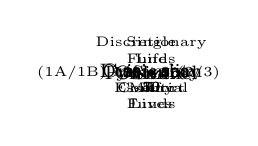
\begin{tikzpicture}[scale=1]
  \path (0:0cm) coordinate (O); % define coordinate for origin

  % draw the spiderweb
  \foreach \X in {1,...,\D}{
    \draw (\X*\A+90:0) -- (\X*\A+90:\L);
  }

  \foreach \Y in {0,...,\U}{
    \foreach \X in {1,...,\D}{
      \path (\X*\A+90:\Y*\R/\U) coordinate (D\X-\Y);
      \fill (D\X-\Y) circle (1pt);
    }
%    \draw [opacity=0.3] (90:\Y*\R/\U) \foreach \X in {1,...,\D}{
%        -- (\X*\A+90:\Y*\R/\U)
%    } -- cycle;
  }
  \foreach \X in {1,...,\D}{
    \path (\X*\A+90:5.7*\R/\U) coordinate (D\X-T);
  }
  \foreach \Y in {0,...,\UU}{
    \foreach \X in {1,...,\D}{
      \path (\X*\A+90:\Y*\R/\UU) coordinate (D\X--\Y);
    }
  }
  
  \path (D5-T) node (L1) {\scriptsize Personnel};
  \draw (D5-5) node[left] {\tiny (1A/1B) 100};
  \draw (D5-5) node[right] {\tiny 0 (2/3)};
  \draw (D5-4) node[left] {\tiny 75};
  \draw (D5-4) node[right] {\tiny 25};
  \draw (D5-3) node[left] {\tiny 50};
  \draw (D5-3) node[right] {\tiny 50};
  \draw (D5-2) node[left] {\tiny 25};
  \draw (D5-2) node[right] {\tiny 75};
  \draw (D5-1) node[left] {\tiny 0};
  \draw (D5-1) node[right] {\tiny 100};
  
  \path (D4-T) node (L2) {\scriptsize Dynamism};
  \draw (D4-5) node[below] {\tiny 1};
  \draw (D4-4) node[below] {\tiny 5};
  \draw (D4-3) node[below] {\tiny 10};
  \draw (D4-2) node[below] {\tiny 30};
  \draw (D4-1) node[below] {\tiny 50};
  
  \path (D3-T) node (L3) {\scriptsize Culture};
  \draw (D3-5) node[left] {\tiny 10};
  \draw (D3-4) node[left] {\tiny 30};
  \draw (D3-3) node[left] {\tiny 50};
  \draw (D3-2) node[left] {\tiny 70};
  \draw (D3-1) node[left] {\tiny 90};
  
  \path (D2-T) node (L4) {\scriptsize Size};
  \draw (D2-5) node[right] {\tiny 300};
  \draw (D2-4) node[right] {\tiny 100};
  \draw (D2-3) node[right] {\tiny 30};
  \draw (D2-2) node[right] {\tiny 10};
  \draw (D2-1) node[right] {\tiny 3};
  
  \path (D1-T) node (L5) {\scriptsize Criticality};
  \draw (D1-5) node[below, align=center, font=\tiny] {Many\\Lives};
  \draw (D1-4) node[above, align=center, font=\tiny] {Single\\Life};
  \draw (D1-3) node[below, align=center, font=\tiny] {Essential\\Funds};
  \draw (D1-2) node[above, align=center, font=\tiny] {Discretionary\\Funds};
  \draw (D1-1) node[below, align=center, font=\tiny] {Comfort};
    
  \draw [color=blue,line width=1.5pt,opacity=0.5]
    (D1--10) --
    (D2--14) --
    (D3--15) --
    (D4--40) --
    (D5--10) -- cycle;

\end{tikzpicture}
\caption{Boehms stjerne-model}
\label{boehms:stjerne}
\end{figure}
}

\begin{description}
\info{Personnel}{beskriver projektgruppens medlemmers ''niveau'' i relation til programmering.
Denne inddeling sker efter Cockburns skala \cite[Tabel 2]{boehm}, der beskriver niveau i relation til det der skal produceres.}
{Vi har i projektgruppen vurderet at alle gruppens medlemmer er på niveau 2 eller 3.}

\info{Dynamism}{angiver i hvilken grad det forventes at der opstår ændringer i et projekts kravspecifikation.
Det fortæller altså i hvilken grad projektgruppen skal være i stand til at tilpasse sig forandringer i krav.}
{Da vi arbejder problembaseret, tages der udgangspunkt i nogle simple og konkrete krav, der i løbet af projektperioden kun vil blive yderligere præciseret.}

\info{Culture}{er en vurdering af hvorvidt en projektgruppes medlemmer trives bedst med kaos eller orden.
På skalaen angives ''hvor meget'' kaos gruppen trives med.}
{Projektgruppens medlemmer har hver især vurderet hvor de ligger på skalaen.
Gennemsnittet af disse vurderinger er på 69,2\%.}

\info{Size}{udtaler sig udelukkende om størrelsen på den gruppe der skal arbejde på et projekt.}
{Projektgruppen består af 6 personer.}

\info{Criticality}{beskriver ''hvor vigtigt'' det er at det endelige produkt er fungerende og lever op til alle krav.
Skalaen angiver denne vigtighed i form af hvilken effekt det har hvis dette ikke er tilfældet.}
{Da den robot, som er projektets mål, ikke skal sættes i produktion, vil den aldrig have højere betydning end \textbf{Comfort} på skalaen.
Det er naturligvis et mål for projektgruppen at have en fungerende robot ved semestrets afslutning.
Men da den tekniske forståelse, som er et biprodukt af det udviklede, ligeledes udbygges, vurderer vi det ikke som kritisk hvis robotten ikke er fuldt fungerende.}
\end{description}

Ud fra modellen (\cref{boehms:stjerne}) ses det at projektgruppen med fordel kan vælge en agil metode til projektarbejdet, da plottet ligger nærmest midten for næsten alle punkter.
Det eneste punkt der ikke direkte anbefaler en agil tilgang er \emph{Dynamism}.
Dog påpeger Boehm og Turner \cite[side 2]{boehm} at dette ikke er et problem:
\quoter{Boehm og Turner}{``For Dynamism, agile methods are at home with 
both high and low rates of change, but plan-driven 
methods prefer low rates of change.''} 
Altså har få krav ikke betydning for valget mellem en agil og en traditionel metode.
Vi kan nu skifte fokus til valg af en specifik agil metode.
I det følgende afsnit gives en kort beskrivelse af udvalgte agile metoder.